\chapter{Математическая модель и программный пакет для анализа динамики транспорта дейтерия в вольфраме}\label{ch:ch2}

Данная глава посвящена описанию основных математических уравнений, обобщающих раздел~\cref{subsec:ch1/sec3/subsec2} и формирующих модель транспорта изотопов водорода в материалах. Кратко представлена схема численного решения использованных уравнений методом конечных элементов, реализованная в программном пакете FESTIM. Приведены детали имплементации кинетической модели, явно учитывающей поверхностные процессы, которая не была ранее реализована в коде. Также описаны результаты верификации и валидации, демонстрирующие корректность реализации и надежность имплементированной модели.

\section{Математическая модель}\label{sec:ch2/sec1}

\subsection{Транспорт изотопов водорода}

В разделе~\cref{sec:ch1/sec3} было продемонстрировано, что удержание изотопов водорода в материала является сложным процессом, определяемым множеством элементарных механизмов взаимодействия, как диффузия, взаимодействие с дефектами и т.д. Учет всех возможных процессов представляет из себя комплексную задачу, полноценная реализация которой маловероятна в настоящее время. В силу этого применяют методы и модели, позволяющие упростить рассмотрение, учитывая при этом наиболее важные механизмы взаимодействия.

Распространенный подход по анализу пространственно-временной эволюции концентрации изотопов водорода в материалах основан модели Макнабба и Фостера~\cite{McNabb1963}. Основные результаты в настоящей работе были получены для случая одного изотопа (дейтерия) в вольфраме, поэтому дальнейшее описание модели будет ограничено соответствующим образом. Обобщение модели на случай нескольких изотопов проводится путем дублирования основных выражений для каждого типа атомов с незначительными изменениями в дефиниции процессов захвата и выхода из дефектов~\cite{Schmid2014}. В основе модели лежит разделение растворенного водорода на две фракции: подвижные атомы с концентрацией \( \cm(\mathbf{x},t) \), свободно диффундирующие по межузельным положениям, и неподвижные с концентрацией \( \ct(\mathbf{x},t) \), захваченные в дефекты разного сорта. Данный подход справедлив в приближении малой концентрации растворенного водорода и дефектов по сравнению с концентрацией атомов решетки материала, что позволяет рассматривать диффузию независимо от остальных процессов. В общем виде распределение концентрации подвижных атомов в момент времени \( t \) в точке \( \mathbf{x} \) геометрической области \( \Omega \), соответствующей объему материала, удовлетворяет следующей системе уравнений:
\begin{subequations}
    \label{eq:ch2/mobile_conc}
    \begin{align}
        \frac{\partial \cm}{\partial t} & = -\nabla \cdot \mathbf{J} - \sum \limits_i \frac{\partial \cti}{\partial t} + \sum \limits_j S_j, \label{eq:ch2/mobile_conc_a} \\
        \mathbf{J}                      & = -D \left( \nabla \cm + \frac{\cm Q^*}{\kBT^2} \nabla T \right). \label{eq:ch2/mobile_conc_b}
    \end{align}
\end{subequations}
Первое слагаемое в правой частиц уравнения~\eqref{eq:ch2/mobile_conc_a} определяет массоперенос за счет совместного влияния градиентов концентрации (закон Фика) и температуры (эффект Соре). Второй член является реакционным слагаемым, характеризующим обменный процесс между фракциями подвижных и захваченных в дефекты \(i\)-типа атомов. Последнее слагаемое учитывает совокупность объемных источников/стоков подвижных атомов со скоростью генерации/поглощения (\( S_j(\mathbf{x},t) \) в \si{\per\meter\cubed\per\second}) за счет таких процессов, как имплантация, распад/генерация трития и т.д. В уравнении массопереноса возможно также учесть адвекцию, которая играет ключевую роль при моделировании распространения водорода в движущейся жидкости~\cite{Dark2021} или в процессе формирования пленок соосаждения~\cite{Krat2020_2}. Однако в настоящей работе данный эффект не рассматривается. Параметры термоактивируемых процессов определяются из пространственно-временной эволюции поля температуры \( T(\mathbf{x},t) \).

В ряде расчетов, проведенных в настоящей работе, учитывался процесс имплантации при облучении поверхности потоком частиц с плотностью \( \Gamma \) (в \si{\per\meter\squared\per\second}), который в общем виде описывается следующим выражением:
\begin{equation}
    \label{eq:ch2/impl_source}
    S(\mathbf{x},t)=\Gamma(t)\varphi(\mathbf{x}),
\end{equation}
где \( \varphi(\mathbf{x}) \) "--- пространственное распределение внедренных частиц, \si{\per\meter}.
\nomenclature[P, 31]{\( S \)}{Объемный источник/сток подвижных атомов, \si{\per\meter\cubed\per\second}}
\nomenclature[P, 32]{\(\Gamma\)}{Плотность потока атомов во время облучения, \si{\per\meter\squared\per\second}}
\nomenclature[P, 33]{\(\varphi\)}{Пространственное распределение внедренных частиц, \si{\per\meter}}

Реакционное слагаемое в выражении~\eqref{eq:ch2/mobile_conc_a} определяется процессами захвата и выхода из ловушек. Рассматриваются насыщаемые неподвижные центры захвата, вмещающие один атом водорода. Предполагается, что дефекты изолированы, т.е. они не образуют протяженную сеть, а транспорт водорода между ними осуществляется посредством диффузии. Влиянием подвижности дефектов, временной эволюции их концентрации~\cite{Dark2024} и наличия ненасыщаемых дефектов~\cite{Zibrov2024} на транспорт водорода пренебрегается. Каждому типу дефектов ставится в соответствие концентрация захваченных в него атомов водорода (\( \cti(\mathbf{x},t) \)), константы скорости захвата (\( \nu_{\mathrm{t},i}(T) \)) и освобождения (\( \nu_{\mathrm{dt},i}(T) \)) и концентрация дефектов (\( n_{\mathrm{t},i}(\mathbf{x}) \) в \si{\per\meter\cubed}). Временная эволюция концентрации атомов водорода, захваченных в тип дефекта \( i \), определяется из:
\begin{equation}
    \frac{\partial \cti}{\partial t} = \nu_{\mathrm{t},i} \cm (n_{\mathrm{t},i} - \cti) - \nu_{\mathrm{dt},i} \cti, \label{eq:ch2/trapped_conc}
\end{equation}
Первое слагаемое в правой части уравнения определяет объемный сток подвижных атомов за счет захвата в дефекты типа \( i \), величина которого зависит от локальной концентрации подвижных атомов и количества незанятых дефектов. Источником подвижных атомов является второе слагаемое, характеризующее скорость выхода атомов из дефекта типа \( i \). Важно заметить, что во втором слагаемом отсутствуют факторы, учитывающие число свободных межузельных положений или наличие соседних дефектов, что обосновывается рассмотрением малой концентрации изолированных дефектов по сравнению с плотностью атомов в решетке материала. Помимо этого, дифференциальное уравнение не учитывает переходы между энергетическими уровнями в одном дефекте, т.н. многочастичный захват. Как показывают результаты численного моделирования~\cite{Schmid2017}, в случае рассмотрения проблемы для одного изотопа водорода совокупность энергетических уровней в центре захвата может быть заменена равным количеством абстрактных дефектов с разными барьерами выхода из них.

Константы скорости процессов задаются на основе закона Аррениуса с соответствующими энергиями активации захвата в дефект (\( E_{\mathrm{t},i} \)) и освобождения из него (\( E_{\mathrm{dt},i} \)):
\begin{subequations}
    \label{eq:ch2/trapping_detrapping_rates}
    \begin{align}
        \nu_\mathrm{t}(T)  & = \nu_{\mathrm{t},0} \exp \left( -\frac{E_\mathrm{t}}{\kB T} \right),    \\
        \nu_\mathrm{dt}(T) & = \nu_{\mathrm{dt},0} \exp  \left( -\frac{E_\mathrm{dt}}{\kB T} \right).
    \end{align}
\end{subequations}
Классическим подходом, позволяющим минимизировать число свободных параметров в модели, является определение константы скорости захвата на основе коэффициента диффузии и параметров кристаллической решетки материала:
\begin{equation}
    \nu_\mathrm{t}(T) \approx \frac{D(T)}{\lambda_\mathrm{IS}^2n_\mathrm{IS}},
\end{equation}
где \(\nu_{\mathrm{t},0}\approx D_0/ (\lambda_\mathrm{IS}^2n_\mathrm{IS})\); \( n_\mathrm{IS} \) "--- объемная концентрация межузельных положений, \si{\per\meter\cubed}; \( \lambda_\mathrm{IS} \) "---  характерное расстояние между межузельными положениями, \si{\meter}. Для объемно-центрированной кубической решетки вольфрама наиболее энергетически выгодными межузельными положениями являются тетраэдрические положения, число которых вблизи атома решетки равно 6, соответственно концентрация межузельных положений \( n_\mathrm{IS} \approx \SI{3.79e29}{\per\meter\cubed} \) при концентрации вольфрама \( n_\mathrm{W}\approx\SI{6.31e28}{\per\meter\cubed} \). Характерное расстояние между такими положениями \( \lambda_\mathrm{IS}=\SI{1.1e-10}{\meter} \). Предэкспоненциальный множитель константы скорости выхода из дефектов обычно полагается равным характерной частоте тепловых колебаний атомов водорода: \( \nu_{\mathrm{dt},0} \approx \nu_0 \approx \SI{e13}{\per\second} \)~\cite{Heinola2010, Fernandez2015}.

\nomenclature[P, 34]{\( n_\mathrm{t} \)}{Концентрация дефектов, \si{\per\meter\cubed}}
\nomenclature[P, 35]{\( n_\mathrm{IS} \)}{Концентрация межузельных положений атома водорода в решетке материала, \si{\per\meter\cubed}}
\nomenclature[P, 36]{\( \nu_0 \)}{Частота тепловых колебаний атома водорода в межузельном положении или дефекте, \si{1\per\second}}
\nomenclature[P, 37]{\( \lambda_\mathrm{IS} \)}{Расстояние между двумя межузельными положениями, \si{\meter}}
\nomenclature[P, 38]{\( \Omega \)}{Геометрическая область пространства}
\nomenclature[P, 39]{\( \partial\Omega \)}{Граница геометрической области}
\nomenclature[P, 40]{\( t \)}{Время, \si{\second}}

Наиболее детальное описание процессов, происходящих на открытых поверхностях исследуемого объема (границе геометрической области \( \partial\Omega \)), дается в рамках модели, явно учитывающей эволюцию концентрации адсорбированного водорода (\( \csurf(\mathbf{x}_s,t) \)). Пространственно-временное распределения поверхностной концентрации может быть определено на основе аналогичной реакционно-диффузионной модели, определенной в подпространстве коразмерности 1\footnote{В зависимости от размерности геометрической области, в которой рассматривается задача транспорта водорода, размерность соответствующей области для задачи о переносе поверхностной концентрации будет на единицу меньше.}. Однако в условиях взаимодействия плазмы с материалами нет необходимости учитывать все процессы. В частности, экспериментальные и теоретические работы показывают, что диффузия водорода по поверхности различных материалов энергетически более выгодна и происходит быстрее, чем другие поверхностные (как десорбция) и объемные механизмы. В связи с этим предполагается, что диффузия будет приводить к распределению поверхностной концентрации адсорбированных атомов значительно быстрее, чем характерное время изменения других величин. Учитывая <<быстрый характер>> диффузии по поверхности, также делается допущение о неявном влиянии центров захвата на поверхности, учет которых осуществляется за счет энергетических барьеров, определяющих вероятности процессов. Учитывая описанные приближения, основное уравнение, определяющее изменение поверхностной концентрации сводится к:
\begin{equation}
    \dfrac{d \csurf}{d t} = J_{\mathrm{bs}} - J_{\mathrm{sb}} + \Jvs, \label{eq:ch2/adsorbed_conc}
\end{equation}
где \( J_{\mathrm{bs}} \) "--- плотность потока атомов из приповерхностной области на поверхность, \si{\per\meter\squared\per\second}; \( J_{\mathrm{sb}} \)  "--- плотность потока атомов с поверхности в приповерхностную область, \si{\per\meter\squared\per\second}; \( J_{\mathrm{vs}}=J_{\mathrm{vs}}(T, \csurf, \cm) \) "--- плотность результирующего потока атомов из вакуума на поверхность, \si{\per\meter\squared\per\second}. Последнее слагаемое включает в себя все рассматриваемые механизмы адсорбции и десорбции, в которых участвуют адсорбированные атомы: \( \Jvs = \sum \limits_i J_{\mathrm{ads},i}^s - \sum \limits_j J_{\mathrm{des},j}^s \).

Уравнение связи между поверхностными и объемными процессами представляет собой граничное условие Робина для задачи транспорта водорода:
\begin{equation}
    \label{eq:ch2/surfaceBC}
    \mathbf{J} \cdot \mathbf{n} = \lambda_{\mathrm{IS}}\dfrac{\partial \cm}{\partial t} + J_{\mathrm{bs}} - J_{\mathrm{sb}} - \Jvb,
\end{equation}
где \( \mathbf{n} \) "--- внешняя нормаль к поверхности (границе \( \partial\Omega \)), \( J_{\mathrm{vs}}=J_{\mathrm{vs}}(T, \csurf, \cm) \) "--- плотность результирующего потока атомов из вакуума в приповерхностную область, \si{\per\meter\square\per\second}. Дефиниция этой величины аналогична поверхностной: \( \Jbs = \sum \limits_i J_{\mathrm{ads},i}^b - \sum \limits_j J_{\mathrm{des},j}^b \). Качественным отличием является тот факт, что величина \( \Jvs \) приводит к изменению поверхностной концентрации атомов водорода, когда \( \Jvb \) влияет на концентрацию атомов в приповерхностной области.

Плотности потоков атомов мигрирующих на поверхность и обратно определяются следующим образом~\cite{Hodille2017}:
\begin{subequations}
    \label{eq:ch2/bs_sb_fluxes}
    \begin{align}
        J_\mathrm{bs} & = \nu_{\mathrm{bs}} c_\mathrm{m} \, \left(1-\dfrac{\csurf}{n_\mathrm{surf}}\right), \\
        J_\mathrm{sb} & = \nu_{\mathrm{sb}} \csurf \, \left(1-\dfrac{\cm}{n_\mathrm{IS}}\right),
    \end{align}
\end{subequations}
Константы скорости процессов определяются на основе закона Аррениуса:
\begin{subequations}
    \label{eq:ch2/bs_sb_nus}
    \begin{align}
        \nubs(T) = \nu_{\mathrm{bs},0} \exp \left( -\frac{E_\mathrm{bs}}{\kB T} \right), \label{eq:ch2/nu_bs} \\
        \nusb(T) = \nu_{\mathrm{sb},0} \exp \left( -\frac{E_\mathrm{sb}}{\kB T} \right). \label{eq:ch2/nu_sb}
    \end{align}
\end{subequations}
Стандартным приближением является определение константы скорости выхода на поверхность через коэффициент диффузии. В случае чистой поверхности (\( E_\mathrm{bs}\approx E_\mathrm{D}) \) можно получить достаточно компактное выражение : \( \nu_\mathrm{bs} \approx D \lambda_\mathrm{abs} / \lambda_\mathrm{IS}^2 \), где \( \lambda_\mathrm{abs} = n_\mathrm{surf} / n_\mathrm{IS} \) "--- характерное расстояние между адсорбционным и межузельным положениями, \si{\meter}. Предэкспоненциальный множитель в уравнении~\cref{eq:ch2/nu_bs} полагается равным частоте колебаний атомов водорода \( \nu_0 \). В выражениях~\cref{eq:ch2/bs_sb_fluxes} члены, заключенные в скобки, учитывают возможное достижении предельной концентрации атомов водорода на поверхности и в приповерхностной области. Эти эффекты' удобно описывать степенью покрытия поверхности (\( \theta \)) и степенью заполненности приповерхностной области (\( \beta \)):
\begin{subequations}
    \label{eq:ch2/theta_omega}
    \begin{align}
        \theta & = \frac{\csurf}{n_\mathrm{surf}}, \\
        \beta  & = \frac{\cm}{n_\mathrm{IS}}.
    \end{align}
\end{subequations}

\nomenclature[P, 41]{\( J_{\mathrm{bs}} \)}{Плотность потока атом из приповерхностной области на поверхность, \si{\per\meter\squared\per\second}}
\nomenclature[P, 42]{\( J_{\mathrm{sb}} \)}{Плотность потока атомов с поверхности в приповерхностную область, \si{\per\meter\squared\per\second}}
\nomenclature[P, 43]{\( J_{\mathrm{vs}} \)}{Плотность результирующего потока атомов из вакуума на поверхность, \si{\per\meter\squared\per\second}}
\nomenclature[P, 44]{\( J_{\mathrm{vb}} \)}{Плотность результирующего потока атомов из вакуума в приповерхностную область, \si{\per\meter\squared\per\second}}
\nomenclature[P, 45]{\( \lambda_\mathrm{abs} \)}{Характерное расстояние между адсорбционным и межузельным положениями в кристаллической решетке материала, \si{\meter}}
\nomenclature[P, 46]{\( n_\mathrm{surf} \)}{Поверхностная концентрация адсорбционных положений, \si{1\per\meter\squared}}
\nomenclature[P, 47]{\( \theta \)}{Степень покрытия повехности}
\nomenclature[P, 48]{\( \beta \)}{Степень заполненности приповерхностной области}

Математическое представление всех возможных процессов адсорбции и десорбции представляется нецелесообразным в настоящем разделе, т.к. выбор доминирующих механизмов, регулирующих эволюцию концентрации водорода, зависит от условий проведения конкретного эксперимента. Детальная информация об учитываемых процессах в рамках каждого модельного случая приводится в соответствующих частях работы. К тому же, применение детальной модели, учитывающей кинетику процессов не всегда необходимо. Как показано в главе~\cref{ch:ch4}, поверхностные процессы могут несущественно влиять на транспорт водорода при импульсных тепловых нагрузках с миллисекундной длительностью

Распространенным приближением является случай локального равновесия процессов вблизи поверхности (см. раздел~\cref{subsec:ch1/sec3/subsec2}). В рамках данного приближения оправдано применение коэффициента рекомбинации \( K_\mathrm{r} \) на поверхности, определяющего плотность потока десорбирующихся частиц с поверхности (граничное условие Неймана). Когда скорость рекомбинация на поверхности происходит значительно быстрее процессов в объеме, возможна редукция к граничному условию Дирихле с нулевым значением концентрации подвижных атомов на границе. Помимо этого, в части задач применялось однородное граничное условие Неймана. В совокупности были использованы три дополнительных граничных условия, применение которых определялось условиями рассматриваемой проблемы:
\begin{subequations}
    \begin{align}
        \mathbf{J} \cdot \mathbf{n} & = -K_\mathrm{r} \cm^2 \label{eq:ch2/recombination_BC}, \\
        \mathbf{J} \cdot \mathbf{n} & = 0 \label{eq:ch2/zero_flux_BC},                       \\
        \cm                         & = 0 \label{eq:ch2/zero_conc_BC}.
    \end{align}
\end{subequations}
Уравнения~\cref{eq:ch2/mobile_conc,eq:ch2/trapped_conc,eq:ch2/adsorbed_conc} дополнялись соответствующими начальными условиями.

\subsection{Перенос тепла}

Из-за многочисленных процессов, которые активируются термически, важно иметь точное температурное поле. Более того, большинство компонентов токамака, обращенных к плазме, подвергаются воздействию интенсивных тепловых потоков и активно охлаждаются, что приводит к появлению температурных градиентов. В связи с этим, неотъемлемой частью моделирования транспорта водорода является определение пространственно-временной эволюции поля температур \( T(\mathbf{x},t) \). Уравнение, описывающее перенос тепла в геометрической области \( \Omega \), определяется следующим образом:
\begin{align}
    \label{eq:ch2/heat_equation}
    \rho C_P \frac{\partial T}{ \partial t} & = -\nabla \cdot \mathbf{J}_q + \sum \limits_i Q_i, \\
    \mathbf{J}_q                            & = -\kappa \nabla T,
\end{align}
где \( \rho \) "--- плотность материала, \si{\kilo\gram\per\meter\cubed}; \( C_P=C_P(T) \) "--- удельная теплоемкость материала, \si{\joule\per\kilo\gram\per\kelvin}; \( \kappa=\kappa(T) \) "--- теплопроводность материала, \si{\watt\per\meter\per\kelvin}; \( Q_i \) "--- объемный источник мощности, \si{\watt\per\meter\cubed}. Теплофизические свойства в общем случае полагаются зависящими от температуры. В уравнении~\cref{eq:ch2/heat_equation} перенос тепла определяется исключительно законом Фурье, т.к. эффекты, связанные с переносом тепла за счет диффузионной теплопроводности, вносят гораздо меньший вклад~\cite{Martinez2021}.

В работе используются неоднородные граничные условия типа Дирихле и Неймана для определения температуры и плотности потока тепла на границе области \( \partial \Omega \):
\begin{subequations}
    \begin{align}
        \mathbf{J}_q \cdot \mathbf{n} & = q(\mathbf{x}, t) \label{eq:ch2/heat_bc_Neumann},  \\
        T                             & = f(\mathbf{x},t) \label{eq:ch2/heat_bc_Dirichlet},
    \end{align}
\end{subequations}
где \(q\) и \(f\) произвольные функции пространственных координат и времени. В каждой задаче также задавалось начальное распределение температуры.

\nomenclature[P, 49]{\( \rho \)}{Плотность материала, \si{\kilo\gram\per\meter\cubed}}
\nomenclature[P, 50]{\( C_P \)}{Удельная теплоемкость материала, \si{\joule\per\kilo\gram\per\kelvin}}
\nomenclature[P, 51]{\( \kappa \)}{Теплопроводность материала, \si{\watt\per\meter\per\kelvin}}
\nomenclature[P, 52]{\( Q \)}{Объемный источник мощности, \si{\watt\per\meter\cubed}}
\nomenclature[P, 53]{\( q \)}{Плотность мощности на границе, \si{\watt\per\meter\squared}}

\section{Программный пакет FESTIM}\label{sec:ch2/sec2}

Беря во внимание нелинейность рассматриваемой системы дифференциальных уравнений в частных производных, получение аналитического решения возможно только в отдельных случаях, зачастую требующих упрощения математической проблемы. Проведение подробного анализа возможно на основе численного моделирования. Существует ряд программных пакетов, разработанных непосредственно для решения задачи транспорта водорода, дополненной уравнением теплопроводности. В зависимости от изначальной цели разработки, данные коды поддерживают разную степень детализированности модели транспорта, размерность пространства, в котором ставится задача, и используют разные методы численного решения. Важной особенностью также является доступность вычислительного инструмента, т.к. большинство программных пакетов для моделирования транспорта изотопов водорода в материалах применяется внутри отдельных исследовательских групп. Программный пакет FESTIM (Finite element simulation of tritium in materials) является одним из немногих свободно распространяемых кодов (лицензия Apache-2.0), позволяющих моделировать транспорт изотопов водорода в одно-/дву-/трехмерной геометрии, включающей несколько материалов, и с возможностью учета физических эффектов, не ограниченных списком, приведенным в предыдущем разделе~\cite{Kulagin2024}.

Для решения системы дифференциальных уравнений в частных производных в коде FESTIM применяется метод конечных элементов (МКЭ), позволяющий исследовать проблему с высокой точностью как на микроскопическом, так и на макроскопическом пространственно-временном масштабе в сложной геометрии~\cite{Nordlund2014}. Программная реализация МКЭ осуществляется с помощью свободно распространяемой библиотеки FEniCS~\cite{FEniCS}, предоставляющей интерфейс для постановки и решения различных задач в частных производных на языках программирования Python и C++. FESTIM обеспечивает более высокий уровень абстракции, чем FEniCS, предоставляя окружение для специализированного решения задач транспорта изотопов водорода и теплопереноса, реализованное на языке программирования Python. Открытость исходного кода и гибкость используемых библиотек позволяет также адаптировать FESTIM для решения конкретной задачи при учете физических процессов, не реализованных исходно в коде.

\nomenclature[A, 13]{МКЭ}{Метод конечных элементов}
\nomenclature[A, 14]{FESTIM}{Код для моделирования транспорта трития в материалах (Finite element simulation of tritium in materials)}

Основная идея МКЭ заключается в дискретизации рассматриваемой области \( \Omega \) на совокупность конечных элементов, в каждом из которых искомое решение уравнения в частных производных аппроксимируется гладкой функцией. Учитывая, что задачи~\cref{eq:ch2/mobile_conc,eq:ch2/heat_equation} относятся к параболическому типу, далее будет приведено краткое описание подхода к решению только задачи транспорта изотопов водорода, реализованном в коде FESTIM. Переход к дискретному представлению проблемы осуществляется с рассмотрения слабой формулировки (вариационной формы), позволяющей расширить класс функций в котором ищется приближенное решение начально-краевой задачи. Вариационная форма получается умножением обеих частей уравнения~\cref{eq:ch2/mobile_conc_a} на тестовую функцию \( v_\mathrm{m} \), обращающуюся в нуль на участке \( \partial \Omega_\mathrm{D} \subset \partial \Omega \), где определены условия типа Дирихле, и последующим интегрированием по области \( \Omega \)~\cite{FEniCS_book}:
\begin{equation}
    \label{eq:ch2/mobile_form}
    \int\limits_\Omega \frac{\partial \cm}{\partial t} v_\mathrm{m} \, dx = \int\limits_\Omega \mathbf{J} \cdot \nabla v_m \, dx - \int\limits_{\partial \Omega_\mathrm{N}} (\mathbf{J}\cdot \mathbf{n}) v_\mathrm{m} \, ds + \int\limits_\Omega S_\Sigma v_\mathrm{m} \, dx,
\end{equation}
где \( dx \) "--- элемент объема; \( ds \) "--- элемент поверхности; \( \Omega_\mathrm{N} \) "--- участок границы области, где определены заданы условия типа Неймана и Робина: \( \partial \Omega = \partial \Omega_\mathrm{D} \cup \partial \Omega_\mathrm{N} \), \( \partial \Omega_\mathrm{D} \cap \partial \Omega_\mathrm{N} = \varnothing \); \( S_\Sigma \) обозначает совокупность всех объемных источников. Дискретизация производной по времени проводится на основе неявного метода Эйлера:
\[
    \frac{\partial \cm}{\partial t} \approx \frac{\cm(t) - \cm(t-\Delta t)}{\Delta t},
\]
где \( \Delta t \) "--- шаг дискретизации по времени, \( \cm(t-\Delta t) \) "--- известное значение функции на предыдущем шаге. Далее будем считать, что вариационная форма справедлива в дискретном подпространстве конечных элементов, формируемом разбиением области \( \Omega \). В качестве базовых элементов для концентрации подвижных атомов водорода в коде FESTIM используются линейные непрерывные элементы Лагранжа (CG1).

При учете взаимодействия с дефектами (уравнение~\cref{eq:ch2/trapped_conc}) создается отдельная тестовая функция \( v_{\mathrm{t},i} \) для концентрации водорода, захваченного в дефект каждого типа. Соответствующая вариационная форма определяется аналогично предыдущему случаю:
\begin{equation}
    \label{eq:ch2/trapped_form}
    \int\limits_\Omega \frac{\partial \cti}{\partial t} v_\mathrm{t} \, dx = \int\limits_\Omega \left( \nu_{\mathrm{t},i} \cm (n_{\mathrm{t},i} - \cti) - \nu_{\mathrm{dt},i} \cti \right) v_{\mathrm{t},i} \, dx.
\end{equation}
Предусматривается возможность использования как линейных непрерывных элементов Лагранжа (CG1), так и линейных разрывных элементов Лагранжа (Галеркина, DG1). Снятие условия на непрерывность функции позволяет иногда избежать развития осцилляций численного решения вблизи границ элементов, например, при рассмотрении кусочно-гладких профилей дефектов.

Имплементация модели, учитывающая кинетику процессов на поверхности, была проведена в рамках настоящей работы. В текущей версии кода (1.4) моделирование процессов на поверхности возможно только в нульмерном приближении при совместном решении задачи транспорта в одномерном приближении. Однако это упрощение не ограничивает существенно применимость модели, поскольку типичные лабораторные эксперименты (ТДС, эксперименты по наводораживанию и т.д.) обычно могут быть описаны в рамках одномерного приближения. Переход к слабой формулировке возможен путем умножения уравнения~\cref{eq:ch2/adsorbed_conc} на тестовую функцию \( v_\mathrm{s} \) и интегрирования по границе области:
\begin{equation}
    \label{eq:ch2/adsorbed_form}
    \int\limits_{\partial \Omega_\mathrm{N}} \frac{\partial \csurf}{\partial t} v_\mathrm{s} \, ds = \int\limits_{\partial \Omega_\mathrm{N}} \left( \Jbs - \Jsb + \Jvs \right) v_\mathrm{s} \, ds.
\end{equation}
Данная процедура повторяется для каждой из границ расчетной области, на которой рассматривается эволюция концентрации адсорбированных атомов. Учитывая нульмерность модели, пробная и тестовые функции определены в пространстве вещественных чисел.

Объединение выражений~\cref{eq:ch2/mobile_form,eq:ch2/trapped_form,eq:ch2/adsorbed_form} приводит в общем случае к нелинейной вариационной задаче вида:
\[
    F(\mathbf{c};\mathbf{v})=0,
\]
где \( \mathbf{c}=(\cm,c_{\mathrm{t},1},c_{\mathrm{t},2},\ldots,c_{\mathrm{t},n},c_{\mathrm{s},1},c_{\mathrm{s},2}) \); \( \mathbf{v}=(v_\mathrm{m},v_{\mathrm{t},1},v_{\mathrm{t},2},\ldots,v_{\mathrm{t},n},v_{\mathrm{s},1},v_{\mathrm{s},2}) \). Равенство выполняется для любых тестовых функций из соответствующего подпространства. Разложение искомых и тестовых функций по базису подпространства конечных элементов приводит к системе нелинейных алгебраических уравнений относительно коэффициентов разложения. Решение системы уравнений в коде FESTIM осуществляется итерационным методом Ньютона. Стоит отметить, что со стороны пользователя требуется только поставить начально-краевую задачу, когда выбор базисных функций, построение вариационной формы, решение системы нелинейных уравнений, экспорт полученных результатов осуществляются внутри программного пакета.

Проверка корректности реализации численной схемы решения рассматриваемой задачи (верификация) и анализ применимости модели для описания эмпирически наблюдаемых процессов (валидация) являются необходимыми условиями использования любого программного пакета, предназначенного для исследования физических явлений. Любые изменения в коде FESTIM проходят тщательную проверку благодаря системе непрерывной интеграции, включающей сотни автоматических тестов как отдельных модулей, так всего пакета. Набор тестов также проводит верификационные проверки отдельных физических модулей, например блок решения уравнения теплопроводности, методами точных и построенных решений. Описанные в рамках данного раздела математические модели не требует специализированной валидации ввиду их многолетней применимости для описания экспериментальных данных. Тем не менее, валидация кода FESTIM проводится на основе литературных данных для демонстрации надежности. Ключевые тестовые задачи представлены в открытом доступе и обобщены в книге по верификации и валидации кода FESTIM~\cite{FESTIM_VV}.

\section{Верификация и валидация модели, учитывающей процессы на поверхности}\label{sec:ch2/sec3}

Раннее отмечалось, что модель~\cref{eq:ch2/adsorbed_conc}, явно учитывающая эволюцию концентрации адсорбированного водорода, была внедрена в код FESTIM в рамках настоящей работы. Как и все основные модули кода, модель требовала проведения верификации и валидации для демонстрации надежности и корректности реализации. Верификация модели проводилась с помощью метода построенных решений (Method of manufactured solutions, MMS), когда валидация осуществлялась путем воспроизведения результатов четырех экспериментальных работ по накоплению изотопов водорода в различных материалах~\cite{Kulagin2025_IJHE}. Все исходные коды, использованные для проверки корректности имплементации модели, распространяются свободно~\cite{vladimir_kulagin_2025_14738004} и включены в онлайн-книгу с результатами верификации и валидации кода FESTIM~\cite{FESTIM_VV}. Важно отметить, что оригинальный анализ был проведен для версии кода 1.3 и применим для версии 1.4. \fixme{В предстоящей версии 1.5 незначительно \href{https://github.com/festim-dev/FESTIM/pull/941}{изменена} процедура определения аргументов Python-класса модели, соответствующих ее физическим параметрам в уравнении~\cref{eq:ch2/adsorbed_conc}. Данное изменение позволяет более гибко задавать параметры модели и не затрагивает ее физической сути. В рамках данного раздела приведены основные результаты верификации и валидации модели в версии кода 1.5. Все адаптированные коды представлены в открытом доступе [ссылка?].}

\subsection{Верификация модели}\label{sec:ch2/sec3/subsec1}
Верификация модели~\cref{eq:ch2/adsorbed_conc}, учитывающей процессы на поверхности, проводилась с помощью метода построенных решений решений. MMS широко используется для оценки точности численных методов решения систем дифференциальных уравнений в частных производных~\cite{Roache2002,Oberkampf_Roy_2010}. Подход заключается в выборе аналитической функции, лежащей в области определения решения системы заданных уравнений. Затем на основе данной функции определяются параметры объемных источников, начальные и граничные условия, при которых функция становится решением системы. На основе определенных параметров и начально-краевых условий требуется получить численное решение рассматриваемой проблемы. Ошибка между <<построенным>> и численным решениями характеризует точность численного метода.

Рассмотрим упрощенную задачу диффузии в области \( \Omega: x \in [0,L] \cup t \in [0,t_f], \, L=1, \, t_\mathrm{f}=5 \):
\begin{equation}
    \label{eq:ch2/manufactured_diffusion}
    \frac{\partial \cm}{\partial t} = D \frac{\partial^2 \cm}{\partial x^2} + S,
\end{equation}
наряду с которой будем также рассматривать дифференциальное уравнение~\cref{eq:ch2/adsorbed_conc}. Взаимодействие с дефектами не влияет на процессы на поверхности, поэтому этот эффект не учитывается. В качестве <<построенного>> решения выберем следующую функцию:
\begin{equation}
    \label{eq:ch2/manufactured_solution}
    c_\mathrm{m, exact}=1+2x^2+x+2t.
\end{equation}
На левой границе области (\( x=0 \)) зададим уравнение~\cref{eq:ch2/surfaceBC}, а на правой (\( x=L \)) потребуем выполнения равенства:
\begin{equation}
    \cm(x=L, t)=c_\mathrm{m, exact}(x=L, t).
\end{equation}
В качестве параметров модели выберем: \( D=7 \), \( \nubs=3 \), \( \nusb = 2n_\mathrm{IS}/n_\mathrm{surf} \), \(n_\mathrm{IS}=20 \), \(n_\mathrm{surf}=5 \), \( \lambda_\mathrm{IS}=2\).

Подстановка выбранных функции и параметров в выражения~\cref{eq:ch2/manufactured_diffusion,eq:ch2/adsorbed_conc} позволяет получить выражение для объемного источника, концентрации адсорбированных атомов (\( c_{\mathrm{s,exact}} \)) и плотности потока из вакуума на поверхность:
\begin{subequations}
    \begin{align}
        S                   & = 2(1-2D),                                                                                                            \\
        c_\mathrm{s, exact} & = n_\mathrm{surf} \dfrac{3(1+2t) + 2\lambda_\mathrm{IS}-D}{2n_\mathrm{IS}+1+2t},                                      \\
        J_{\mathrm{vs}}     & = 2n_\mathrm{surf} \dfrac{6n_\mathrm{IS} - 2\lambda_\mathrm{IS}+D}{(2n_\mathrm{IS}+1+2t)^2} + 2\lambda_\mathrm{IS}-D.
    \end{align}
\end{subequations}
В качестве начальных условий полагаем:
\begin{subequations}
    \begin{align}
        \cm(x, t=0) & = c_\mathrm{m, exact}(x, t=0) \\
        \csurf(t=0) & = c_\mathrm{s, exact}(t=0)
    \end{align}
\end{subequations}
Моделирование проводится на равномерной сетке, состоящей из 1000 элементов, с фиксированным размером временного шага. Оценка точности численного решения (\( c_\mathrm{m, computed} \), \( c_\mathrm{s, computed} \)) проводилась на основе \( L^2 \)-нормы:
\begin{subequations}
    \begin{align}
        E_\mathrm{m} & = \sqrt{ \int\limits_\Omega \left(c_\mathrm{m, exact}-c_\mathrm{m, computed}\right)^2 d\Omega },      \\
        E_\mathrm{s} & = \sqrt{ \int\limits_0^{t_\mathrm{f}} \left(c_\mathrm{s, exact}-c_\mathrm{s, computed}\right)^2 dt }.
    \end{align}
\end{subequations}

На рисунке~\cref{fig:ch2/MMS_a,fig:ch2/MMS_b} приведено сравнение результатов. Численные решения хорошо согласуются с точными: \(E_m = \num{2.28e-5} \) и \( E_\mathrm{s}= \num{4.36e-5} \).
\begin{figure}[ht]
    \centerfloat{
        \hfill
        \subcaptionbox[List-of-Figures entry]{\label{fig:ch2/MMS_a}}{%
            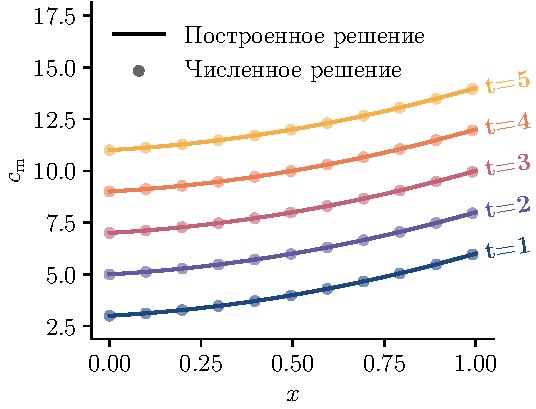
\includegraphics[scale=1]{MMS_a.pdf}}
        \hfill
        \subcaptionbox{\label{fig:ch2/MMS_b}}{%
            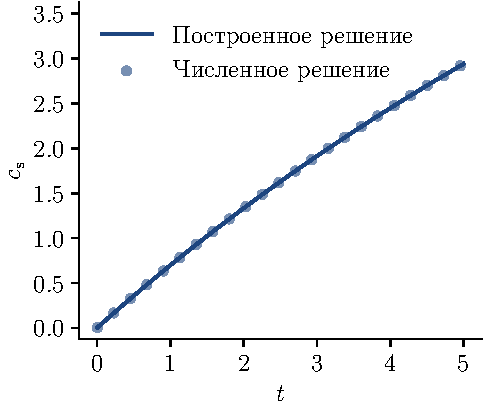
\includegraphics[scale=1]{MMS_b.pdf}} \\
        \subcaptionbox{\label{fig:ch2/MMS_c}}{%
            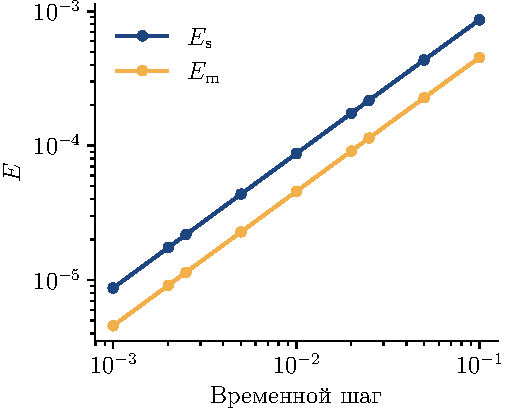
\includegraphics[scale=1]{MMS_c.pdf}}
    }
    \caption{Эволюция профиля концентрации подвижных атомов (a) и временная эволюция концентрации адсорбированных атомов (б) при временном шаге \num{5e-3}; (в) зависимость отклонения численных решений от аналитических}\label{fig:ch2/MMS}
\end{figure}
Учитывая нульмерность уравнения~\cref{eq:ch2/adsorbed_conc}, интерес представляет анализ сходимости по временной дискретизации. Из рисунка~\cref{fig:ch2/MMS_c} видно, что ошибки для обеих переменных линейно спадают с уменьшением временного шага, что ожидаемо ввиду использования схемы Эйлера для аппроксимации временных производных.

\subsection{Валидация модели}\label{sec:ch2/sec3/subsec2}

В этом разделе представлены четыре валидационных теста, использованных для проверки реализованной модели~\cref{eq:ch2/adsorbed_conc}. Они воспроизводят эксперименты по накоплению изотопов водорода в титане, вольфраме и стали EUROFER при облучении поверхности потоком атомов или молекул с низкой энергией. Кроме того, три случая включают сравнение с результатами моделирования, полученными с помощью кодов MHIMS~\cite{Hodille2024} или TESSIM-X~\cite{Schmid2016}. Во всех случаях рассматривался транспорт водорода в одномерном приближении, определяемый законом Фика, а эволюция температуры задавалась по известному закону. С точки зрения моделирования, основным отличием являются разные предположения о процессах, протекающих на поверхности в частном эксперименте.

\subsubsection{Эксперимент по абсорбция протия в титане}
Первый тестовый случай воспроизводит эксперименты по абсорбции протия в титане при различных значениях температуры~\cite{Hirooka1981}. Эксперименты по абсорбции проводились в вакуумной камере при базовом давлении $P_\mathrm{H_2}=\SI{1.3e4}{\pascal}$ с образцами размером $10\times13\times1$ мм. Образцы поддерживались при постоянной температуре в диапазоне от \SI{473}{K} до \SI{923}{K}. В моделировании полагается, что эволюция поверхностной концентрации протия определяется ​​адсорбцией ($J_{\mathrm{ads}}^{\mathrm{H_2}}$) и рекомбинацией ($J_\mathrm{des}^{\mathrm{H_2}}$) молекул~\cite{Shimohata2021}. Таким образом, результирующая плотность потока из вакуума на поверхность в уравнении~\cref{eq:ch2/adsorbed_conc} определяется следующими выражениями:
\begin{subequations}
    \label{eq:ch2/case1_surf_proc}
    \begin{align}
        \Jvs                          & = J_\mathrm{ads}^{\mathrm{H_2}}-J_\mathrm{des}^{\mathrm{H_2}},                                 \\
        J_\mathrm{ads}^{\mathrm{H_2}} & = 2 \, \nu_{\mathrm{ads}}^{\mathrm{H_2}} P_\mathrm{H_2} \, \left(1-\theta_\mathrm{H}\right)^2, \\
        J_\mathrm{des}^{\mathrm{H_2}} & = 2 \, \nu_\mathrm{des}^{\mathrm{H_2}} \, \csurf^2,
    \end{align}
\end{subequations}
где \( \theta_\mathrm{H}=\csurf/n_\mathrm{surf} \) "--- степень покрытия поверхности титана протием; \( \nu_\mathrm{des}^{\mathrm{H_2}}=\nu_\mathrm{des,0}^{\mathrm{H_2}} \exp(-E_\mathrm{des}/k_\mathrm{B} T) \) "--- константа скорости десорбции за счет рекомбинации двух атомов на поверхности. Константа скорости адсорбции определяется как:
\begin{equation}
    \label{eq:ch2/nu_ads_P}
    \nu_{\mathrm{ads}}^{\mathrm{H_2}} = \dfrac{\Phi}{\sqrt{2\pi m_\mathrm{H_2}k_\mathrm{B} T}},
\end{equation}
где \( \Phi = \Phi_0 \exp \left( -E_\mathrm{diss}/\kBT \right) \) "--- коэффициент прилипания; $m_\mathrm{H_2}$ "--- масса молекулы протия, \si{\kilo\gram}. Давление в камере рассчитывается из уравнения состояния идеального газа:
\begin{equation}
    P_\mathrm{H_2} = \left( \frac{P_\mathrm{H_2,0} V_\mathrm{ch}}{k_\mathrm{B} T} + \frac{N_0-N}{2} \right) \frac{k_\mathrm{B} T}{V_\mathrm{ch}},
\end{equation}
где \( P_\mathrm{H_2,0} \) "--- начальное давление в камере, \si{\pascal}; \( V_\mathrm{ch} \) "--- объем камеры, \si{\meter\cubed}; \( N_0 \) "--- начальное число атомов протия в титане; \( N \) "--- действующее число атомов протия в титане. Содержание протия в титане определяется как сумма интегрального числа атомов на поверхности и в объеме.

\nomenclature[P, 54]{\( \nu_\mathrm{ads}^{\mathrm{I_2}} \)}{Константа скорости адсорбции молекул изотопа водорода I из газовой фазы, \si{\per\meter\squared\per\second\per\pascal}}
\nomenclature[P, 55]{\( \nu_\mathrm{des}^{\mathrm{I_2}} \)}{Константа скорости десорбции атомов изотопа водорода I по каналу Ленгмюра-Хиншельвуда, \si{\meter\squared\per\second}}
\nomenclature[P, 56]{\( \nu_\mathrm{des}^{\mathrm{I}} \)}{Константа скорости десорбции атомов изотопа водорода I по каналу Или-Ридила, \si{\per\second}}
\nomenclature[P, 57]{\( \Phi \)}{Коэффициент прилипания}
\nomenclature[P, 58]{\( m_{\mathrm{I}} \)}{Масса молекулы изотопа водорода I, \si{\kilo\gram}}
\nomenclature[P, 59]{\( V \)}{Объем, \si{\meter\cubed}}
\nomenclature[P, 60]{\( N \)}{Число атомов изотопа водорода}
\nomenclature[P, 61]{\( L \)}{Толщина геометрии, \si{\meter}}

Константы скорости переходов между поверхностью и приповерхностной областью определяются в соответствии с законом Аррениуса (уравнения \cref{eq:ch2/bs_sb_nus}). Взаимодействие с центрами захвата не учитывается. Количество межузульных и адсорбционных положений оценивается через объемную концентрацию атомов титана ($n_\mathrm{Ti}$ в \si{\per\meter\cubed}). Начальное содержание протия в титане принимается равным нулю. Моделирование проводилось только для половины геометрии на сетке, состоящей из 1000 равных элементов, с условием симметрии (нулевым потоком) на правой границе и моделью, учитывающей процессы на поверхности, определенной на левой границе.

Для воспроизведения экспериментальных зависимостей была проведена процедура автоматической оптимизации параметров~\cite{Delaporte-Mathurin2021}. Процедура заключается в построении функции ошибки, характеризующей отклонение численных результатов от экспериментальных. В качестве функции ошибки использовалось cреднеквадратическое отклонение по всей выборке. Затем проводится оптимизация параметров для минимизации ошибки между результатами. В рамках работы для этой процедуры применялся алгоритм Недлера-Мида. Параметры $\nu_\mathrm{des,0}$, $E_\mathrm{des}$, $\nu_\mathrm{bs,0}$, $E_\mathrm{bs}$, $\nu_\mathrm{sb,0}$ и $E_\mathrm{sb}$ рассматривалась как свободные. Для первоначального предположения использовались соответствующие значения, представленные в работе~\cite{Shimohata2021}. Совокупность входных параметров обобщена в таблице~\cref{tab:case1_inputs}.

\begin{table}[h]
    \centering
    \begin{threeparttable}
        \caption{\fixme{Входные параметры модели для первого валидационного теста}}
        \label{tab:123}
        \renewcommand{\arraystretch}{1.2}%% Увеличение расстояния между рядами, для улучшения восприятия.
        \def\tabularxcolumn#1{m{#1}}
        \begin{tabular}{|c|c|c|c|c|c|}
            \hline
            $L$, \si{\meter}                                     & $n_\mathrm{Ti}$, \si{\per\meter\cubed}      & $n_\mathrm{IS}$, \si{\per\meter\cubed} & $n_\mathrm{surf}$, \si{\per\meter\squared} & $\lambda_\mathrm{IS}$, \si{\meter}    & $D_0$, \si{\meter\squared\per\second} \\
            \hline
            \num{1.0e-3}                                         & \num{5.66e28}                               & \num{1.69e29}                          & \num{3.90e19}                              & \num{2.29e-10}                        & \num{9.0e-7}                          \\
            \hline
            \hline
            $E_\mathrm{D}$, \si{\electronvolt}                   & $E_\mathrm{des}$, \si{\electronvolt}        & $E_\mathrm{bs}$, \si{\electronvolt}    & $E_\mathrm{sb}$, \si{\electronvolt}        & $E_\mathrm{diss}$, \si{\electronvolt} & $\Phi_0$                              \\
            \hline
            \num{0.538}                                          & \num{0.562}                                 & \num{1.052}                            & \num{1.009}                                & \num{2.06e-2}                         & \num{1.43e-2}                         \\
            \hline
            \hline
            $\nu_\mathrm{des,0}$, \si{\meter\squared\per\second} & $\nu_\mathrm{bs,0}$, \si{\meter\per\second} & $\nu_\mathrm{sb,0}$, \si{\per\second}  & $P_\mathrm{H_2,0}$, \si{\pascal}           & $V_\mathrm{ch}$, \si{\meter\cubed}    &                                       \\
            \hline
            \num{3.41e-11}                                       & \num{2.3}                                   & \num{5.14e9}                           & \num{1.3e4}                                & \num{2.95e-3}                         &                                       \\
            \hline
        \end{tabular}
    \end{threeparttable}
\end{table}

Степень согласия между результатами моделирования и эксперимента количественно определялась с помощью среднеквадратической ошибки:
\begin{equation}
    \mathrm{RMSE} = \sqrt{\dfrac{1}{N} \sum \limits_{i=1}^N(x_{\mathrm{sim},i}-x_{\mathrm{exp},i})^2},
\end{equation}
где $x_{\mathrm{sim},i}$ и $x_{\mathrm{exp},i}$ представляют собой рассчитанные и экспериментальные значения анализируемой величины (в данном случае содержание протия в титане).

Сравнение результатов представлено на рисунке~\cref{fig:ch2/val1}. Достигнуто разумное согласие (\( \mathrm{RMSE}=\num{2.915e-2} \)) между результатами моделирования в коде FESTIM и экспериментальными данными во всем диапазоне температур при использовании одного напора параметров.
\begin{figure}[ht]
    \centerfloat{
        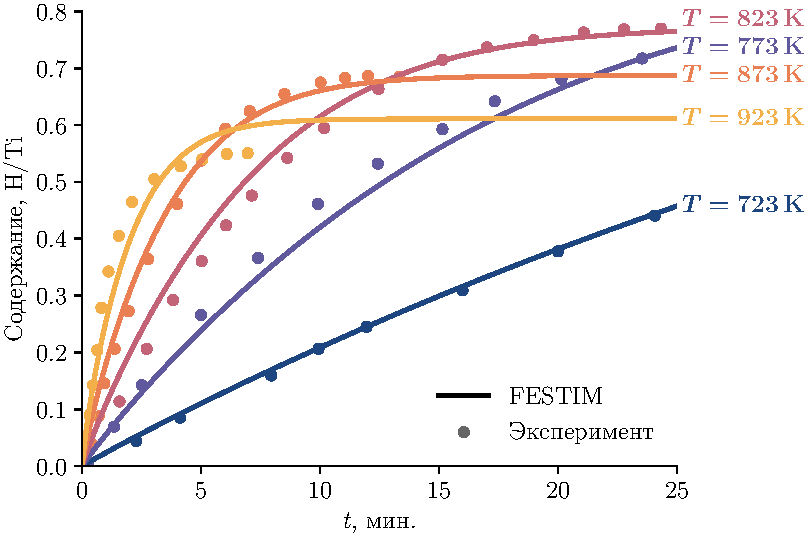
\includegraphics[scale=1]{val1.pdf}
    }
    \caption{Временные зависимости содержания протия в титане при различных температурах}\label{fig:ch2/val1}
\end{figure}

\subsubsection{Эксперимент по адсорбция дейтерия на поверхности оксидированного вольфрама}
Второй валидационный тест воспроизводит экспериментальные результаты по десорбции дейтерия с поверхности окисленного вольфрама~\cite{Dunand2022}. Три монокристаллических образца (толщиной \(L=\SI{2}{\milli\meter}\)) были подготовлены с различной степенью покрытия поверхности кислородом \( \theta_\mathrm{O}=0;~0.5;~0.75 \). Образцы подвергались воздействию потока газа при базовом давлении в камере $P_\mathrm{D_2}=\SI{2e-5}{\pascal}$ и комнатной температуре (\SI{300}{K}). Облучение длилось три тысячи секунд, за которой следовала фаза хранения в течение одного часа. После этого были проведены ТДС-измерения потока десорбированных частиц с постоянной скоростью нагрева равной пять кельвин в секунду.

Следуя работе~\cite{Hodille2024}, предполагается, что эволюция поверхностной концентрации $\csurf$ в настоящей модели определяется адсорбцией дейтерия из газовой фазы и десорбцией молекул с поверхности, аналогично первому тестовому случаю (уравнения~\eqref{eq:ch2/case1_surf_proc}). Константа скорости адсорбции рассчитывается согласно уравнению~\cref{eq:ch2/nu_ads_P} с использованием массы молекулы и парциального давления дейтерия в камере. Полагается, что наличие кислорода на поверхности вольфрама влияет на количество доступных мест адсорбции:
\begin{equation}
    n_\mathrm{surf}(\theta_\mathrm{O}) = n_\mathrm{surf}(0)(1-\theta_\mathrm{O}).
\end{equation}

Согласно расчетам методом DFT, энергия активации десорбции зависит от степени покрытия поверхности~\cite{Piazza2018,Ajmalghan2019,Ferro2023}. Чтобы учесть этот эффект, в работе~\cite{Hodille2024} использовалась следующая константа скорости десорбции:
\begin{subequations}
    \begin{align}
        \nu_\mathrm{des}^{\mathrm{D_2}}   & = \nu_\mathrm{des,0}^{\mathrm{D_2}} \exp \left( -\frac{E_\mathrm{des}(\theta)}{k_\mathrm{B} T} \right), \\
        \nu_\mathrm{des,0}^{\mathrm{D_2}} & = \nu_0\lambda_\mathrm{des}^2,
    \end{align}
\end{subequations}
где $\nu_0$ "--- характерная частота колебаний атомов дейтерия, \si{\per\second}; $\lambda_\mathrm{des}=1/\sqrt(n_\mathrm{surf})$ "--- характерное расстояние между адсорбционным положениями, \si{\meter}. Зависимость энергии активации для десорбции($E_\mathrm{des}$ в \si{\electronvolt}) была аппроксимирована следующим выражением:
\begin{subequations}
    \begin{align}
        E_\mathrm{des}(\theta_\mathrm{D}) & = E_\mathrm{1}(\theta_\mathrm{D})\left( 1-a \exp\left( -b (1-\theta_\mathrm{D}) \right) \right), \label{eq:ch2/case2_Edes} \\
        E_\mathrm{1}(\theta_\mathrm{D})   & = E_0 + \dfrac{\Delta E}{1+\exp\left( \dfrac{\theta_\mathrm{D}-\theta_\mathrm{D,0}}{\delta\theta_\mathrm{D}} \right)}.
    \end{align}
\end{subequations}
Здесь $E_\mathrm{1}$ выражается сигмоидальным распределением и определяет изменение энергии десорбции ниже насыщения. Множитель в скобках в уравнении (\ref{eq:ch2/case2_Edes}) отвечает за экспоненциальное уменьшение энергии десорбции выше насыщения~\cite{Ferro2023, Matveev2018}.

\nomenclature[P, 62]{\( \lambda_\mathrm{des} \)}{Характерное расстояние между адсорбционными положениями, \si{\meter}}

Используются зависящие от температуры (уравнения~\eqref{eq:ch2/bs_sb_nus}) скорости переходов атомов дейтерия между поверхностью и приповерхностной областью. Энергия активации для абсорбции задается в соответствии с расчетами DFT~\cite{Ajmalghan2019, Ferro2023}: $E_\mathrm{bs}\approx E_\mathrm{D}$, с предэкспоненциальныи множителем: $\nu_\mathrm{bs,0}=\nu_0 n_\mathrm{surf} / n_\mathrm{IS}$. Константа скорости абсорбции также полагается зависящей от концентрации дейтеряи на поверхности:
\begin{subequations}
    \begin{align}
        \nusb                 & = \nu_\mathrm{sb,0}\exp\left( -\frac{E_\mathrm{sb}(\theta)}{k_\mathrm{B} T} \right),                          \\
        E_\mathrm{sb}(\theta) & = \frac{E_\mathrm{des}(\theta) - E_\mathrm{diss}}{2} + E_\mathrm{bs} + Q_\mathrm{S}, \label{eq:ch2/case2_Esb}
    \end{align}
\end{subequations}
где $\nu_\mathrm{sb,0} = \nu_0$; $Q_\mathrm{S}=\SI{1}{\electronvolt}$~\cite{Fernandez2015} "--- теплота раствора дейтерия в вольфраме.

Поскольку вероятность абсорбции при комнатной температуре пренебрежимо мала, центры захвата в текущем случае не рассматриваются. Однако для полной постановки задачи транспорта в коде FESTIM требуются задать параметры объемных процессов. Коэффициент диффузии дейтерия в вольфраме определяется путем масштабирования соответствующего коэффициента для протия~\cite{Fernandez2015}. Как и в предыдущем случае, количество межузельных и адсорбционных положений оценивается через объемную концентрацию атомов вольфрама ($n_\mathrm{W}$).

Моделирование проводилось на равномерной сетка из 500 элементов с условием~\cref{eq:ch2/adsorbed_conc} на левой границе ($x=0$) и однородным граничным условием Дирихле на правой ($\cm(x=L)=0$). В начале моделирования предполагается, что концентрация дейтерия в вольфраме равна нулю. Все входные параметры моделирования обобщены в таблицах~\cref{tab:case2_inputs,tab:case2_Edes_params}. Сравнение результатов численных расчетов приведено на рисунке~\cref{fig:ch2/val2}.

\begin{figure}[ht]
    \centerfloat{
        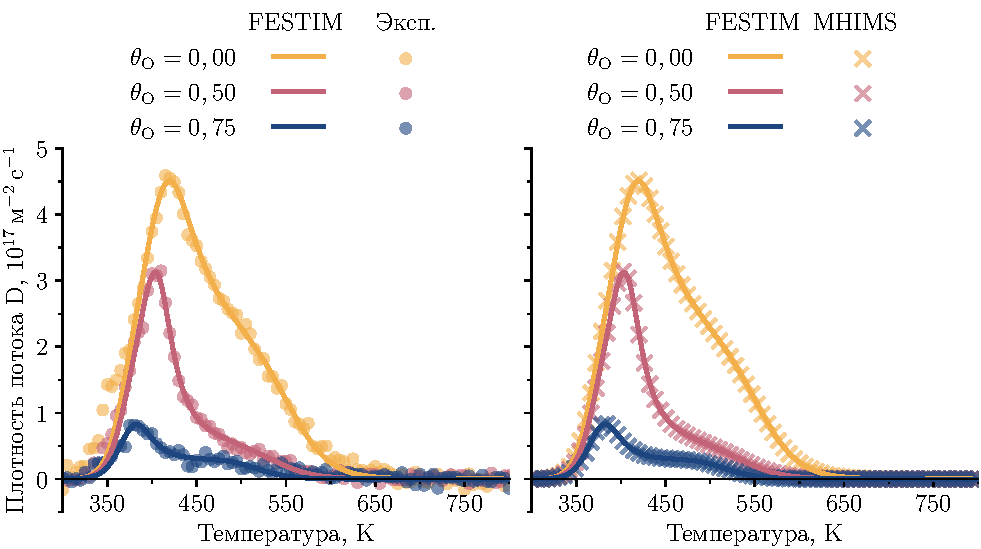
\includegraphics[scale=1]{val2.pdf}
    }
    \caption{ТДС-спектры дейтерия, десорбированного с поверхности вольфрама при различным значениях степени покрытия поверхности кислородом. Сравнение с экспериментальными данными (слева) и численными результатами, полученными в коде MHIMS (справа)}\label{fig:ch2/val2}
\end{figure}

Все зависимости демонстрируют пик в области низких с температур с затяжным высокотемпературным плечом. С увеличением концентрации кислорода на повернхости пик смещается в область более низких температур, а общее количество вышедшего дейтерия спадает из-за меньшего числа доступных мест для адсорбции. Смоделированные зависимости демонстрируют хорошее согласие с экспериментальными данными и прекрасно коррелируют с результатами, полученными в коде MHIMS. Среднеквадратические отклонения между численными результатами и экспериментальными данными находятся на уровне шума и равны \SI{2.1e16}{\per\meter\squared\per\second} при \( \theta_\mathrm{O}=0 \); \SI{8.8e15}{\per\meter\squared\per\second} при \( \theta_\mathrm{O}=0,5 \); \SI{7.2e15}{\per\meter\squared\per\second} при \( \theta_\mathrm{O}=0,75 \).

\subsubsection{Эксперимент по облучению вольфрама низкоэнергетичными атомами дейтерия}
Третий случай проверки воспроизводит результаты МЯР-измерений распределения дейтерия в вольфраме после облучения потоком атомов с низкой энергией~\cite{Markelj2016}. Экспериментальная процедура включала три основные фазы. Поликристаллический образец вольфрама толщиной \(L=\SI{0.8}{\milli\meter}\) был предварительно облучен ионами вольфрама с энергией \SI{20}{\mega\electronvolt} до дозы \SI{7.8e17}{\meter\squared} для создания дефектов в приповерхностном слое. Затем этот предварительно поврежденный образец был подвергнут воздействию облучению низкоэнергетическими (\SI{\approx 0.3}{\electronvolt}) атомами дейтерия с плотностью потока \(\Gamma_\mathrm{D}=\SI{5.8e18}{\per\meter\squared\per\second}\) при температуре образца \SI{600}{\kelvin}. Облучение длилось до тех пор, пока не был достигнута доза \SI{e24}{\per\meter\squared}. На финальном этапе проводилось обезгаживание образца в течение \SI{43}{h} при температуре равной \SI{600}{K}.

В численной модели рассматриваются три процесса на поверхности: адсорбция низкоэнергетических атом ($J_\mathrm{ads}^\mathrm{D}$), десорбция по механизму Ленгмюра-Хиншельвуда ($J_\mathrm{des}^\mathrm{D_2}$) и десорбция по механизму Эли-Ридила ($J_\mathrm{des}^{\mathrm{D}}$). Плотности потока атомов, обусловленные упомянутыми механизмами, определяются на основе выражений:
\begin{subequations}
    \label{eq:ch2/case3_Jvs}
    \begin{align}
        \Jvs                        & = J_\mathrm{ads}^\mathrm{D}-J_\mathrm{des}^\mathrm{D_2}-J_\mathrm{des}^\mathrm{D}, \\
        J_\mathrm{ads}^\mathrm{D}   & = \Gamma_\mathrm{D} \Phi \, \left( 1 - \theta_\mathrm{D} \right),                  \\
        J_\mathrm{des}^\mathrm{D_2} & = 2 \, \nu_\mathrm{des}^\mathrm{D_2} \, \csurf^2,                                  \\
        J_\mathrm{des}^\mathrm{D}   & = \nu_\mathrm{des}^\mathrm{D} \, \csurf,
    \end{align}
\end{subequations}
где \( \nu_\mathrm{des}^\mathrm{D} = \Gamma_\mathrm{D} \sigma_\mathrm{ER} \) "--- константа скорости десорбции за счет рекомбинации адсорбированного и приходящего атомов дейтерия, \si{\per\second}; \( \sigma_\mathrm{exc} \) "--- поперечное сечение процесса, \si{\meter\squared}. Константы скорости остальных процессов задаются в соответствии с законом Аррениуса. Соответствующие Предэкспоненциальные множители: $\nu_\mathrm{des,0}=\nu_0 \lambda_\mathrm{des}^2$, $\nu_\mathrm{bs,0}=\nu_0 n_\mathrm{surf} / n_\mathrm{IS}$ и $\nu_\mathrm{bs,0}=\nu_0$.

\nomenclature[P, 63]{\( \sigma_\mathrm{ER} \)}{Сечение процесса десорбции по каналу Или-Ридила, \si{\meter\squared}}

Для этой задачи используется тот же коэффициент диффузии дейтерия, что и в предыдущем валидационном тесте. Для воспроизведения экспериментальных данных включены пять типов центров захвата: два естественных, равномерно распределенные по всему объему образца, и три индуцированных с сигмоидальным распределением ($\varphi$) внутри поврежденного слоя:
\begin{equation}
    \varphi(x)=\frac{1}{1+\exp\left( \dfrac{x-x_0}{\Delta x} \right)}
\end{equation}
где $x_0=\SI{2.2}{\micro\meter}$, $\Delta x=\SI{0.154}{\micro\meter}$. Скорость захвата во все типы дефектов полагается определяемой диффузией.

На передней поверхности ($x=0$) задается модель, учитывающая все процессы на поверхности, тогда как на противоположной стороне ($x=L$) учитываются только десорбционные члены в системе~\eqref{eq:ch2/case3_Jvs}. Моделирование проводилось на неоднородной сетке (шаг дискретизации меньше у левой границы), включающей 800 элементов. Нулевые начальные условия использовались для концентраций подвижного и адсорбированного H. Чтобы сравнить результаты моделирования с более ранними данными~\cite{Hodille2017}, полученными с помощью кода MHIMS, моделируются только изотермические фазы облучения и десорбции, опуская промежуточные этапы охлаждения/повторного нагрева. Все входные параметры приведены в таблицах~\cref{tab:case3_inputs,tab:case3_traps_params}. Сравнение результатов с данными экспериментов и MHIMS представлено на рисунке~\cref{fig:ch2/val3}.

\begin{figure}[ht]
    \centerfloat{
        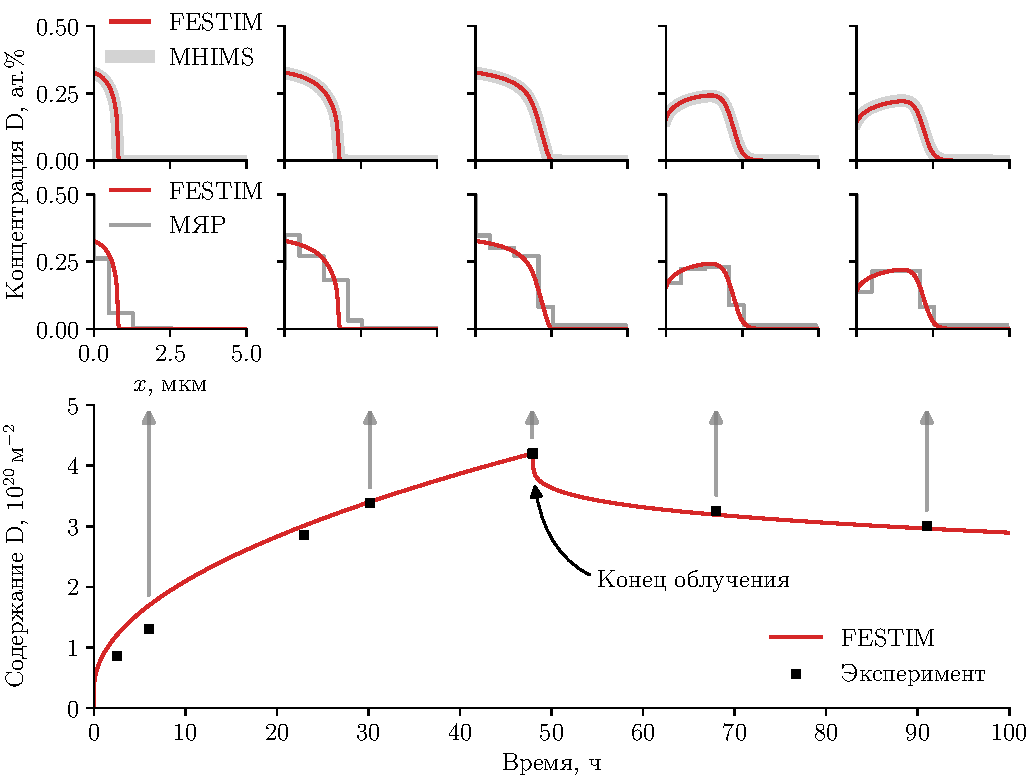
\includegraphics[scale=1]{val3.pdf}
    }
    \caption{Временная эволюция содержания дейтерия в вольфраме (внизу). Сравнение между данными FESTIM и МЯР (в середине) и между данными FESTIM и MHIMS (вверху)}\label{fig:ch2/val3}
\end{figure}

Во время фазы экспозиции содержание дейтерия увеличивается (см. нижний график на рис.~\ref{fig:ch2/val3}), профиль концентрации расширяется по мере заполнения более глубоколежащих дефектов (см. верхний/средний ряд графиков). Во время фазы десорбции наблюдается более медленное снижение накопления из-за наличия ловушек с высокой ($>$\SI{1.5}{\electronvolt}) энергией активации освобождения. Результаты, полученные в коде FESTIM, хорошо согласуются с экспериментальными данными (среднеквадратическое отклонение в величине интегрального накопления \SI{2.1e19}{\per\meter\squared}) и практически совпадают с данными MHIMS.

\subsubsection{Эксперимент по облучению стали EUROFER ионами дейтерия}
Последний валидационный тест посвящен накоплению дейтерия при облучении стали EUROFER ионами с низкой энергией~\cite{Schmid2023_1}. Эксперименты проводились с тремя типами образцов (толщиной \(L=\SI{0.8}{\milli\meter}\)): неповрежденными; предварительно поврежденными ионами вольфрама с энергией \SI{20}{\mega\electronvolt}; предварительно облученными дейтерием и затем поврежденными ионами вольфрама. Эти образцы облучались потоком дейтерия $\approx\SI{9e19}{\meter^{-2}s^{-1}}$ с энергией \SI{5}{\text{эВ/ион}} при давлении газа $P_\mathrm{D_2}=\SI{1}{\pascal}$ и температуре \SI{370}{K}. Время облучения низкоэнергетическим дейтерием в этих экспериментах варьировалось от \SI{48}{\hour} до \SI{143}{\hour}, что приводит к четырем модельным случаям:
\begin{enumerate}[beginpenalty=10000]
    \item Неповрежденный образец, облучение дейтерием длительностью \SI{143}{\hour}.
    \item Поврежденный образец, облучение дейтерием длительностью \SI{48}{\hour}.
    \item Поврежденный образец, облучение дейтерием длительностью \SI{143}{\hour}.
    \item Предоблученный дейтерием поврежденный образец, облучение дейтерием длительностью \SI{48}{\hour}.
\end{enumerate}
После облучения образцы хранились в течение \SI{24}{\hour} при \SI{290}{\kelvin}. После хранения были проведены ТДС-измерения со скоростью нагрева 3 кельвин в минуту до температуры 800 кельвин.

Подобно предыдущему случаю проверки, в кинетическую модель поверхности включены три механизма: диссоциативная адсорбция молекул ($J_\mathrm{ads}^{\mathrm{D_2}}$), рекомбинация молекул ($J_\mathrm{des}^{\mathrm{D_2}}$) и десорбция за счет мгновенной рекомбинации с приходящими ионами ($J_\mathrm{des}^{\mathrm{D}}$). Результирующая плотность потока атомов на поверхность равен:
\begin{subequations}
    \label{eq:ch2/case4_Jvs}
    \begin{align}
        \Jvs                          & = J_\mathrm{ads}^{\mathrm{D_2}}-J_\mathrm{des}^{\mathrm{D_2}}-J_\mathrm{des}^{\mathrm{D}}, \\
        J_\mathrm{ads}^{\mathrm{D_2}} & = 2 \, \nu_\mathrm{ads}^{\mathrm{D_2}} P_\mathrm{D_2} \, \left( 1 - \theta \right)^2,      \\
        J_\mathrm{des^{\mathrm{D_2}}} & = 2 \, \nu_\mathrm{des}^{\mathrm{D_2}} \, \csurf^2,                                        \\
        J_\mathrm{des}^{\mathrm{D}}   & = \nu_\mathrm{des}^{\mathrm{D}} \, \csurf.
    \end{align}
\end{subequations}
Константа скорости адсорбции молекул рассчитывается как во втором и третьем валидационных тестах (уравнение~\cref{eq:ch2/nu_ads_P}). Константа скорости десорбции по каналу Или-Ридила определяется аналогично прошлому тесту, но на основе потока внедренных частиц: \( \Gamma_\mathrm{D}^{\mathrm{impl}}=\Gamma_\mathrm{D}(1-r) \), где \( r \) "--- коэффициент отражения частиц от поверхности.

Переход из растворенного в адсорбированное состояние полагается определяемым диффузией: $E_\mathrm{bs}=E_\mathrm{D}$ и $\nu_\mathrm{bs,0}=D_0/\lambda_\mathrm{IS}$. Количество межузельных и адсорбционных положений рассчитываются на основе концентрации атомов стали ($n_\mathrm{EFe}$). Константа скорости перехода из адсорбированного в растворенное состояние выбирается таким образом, чтобы выполнялся закон Сивертса:
\begin{flalign}
    \label{eq:ch2/case4_ksb}
    \nusb = \nubs \, K_\mathrm{S} \, \sqrt{\frac{\nu_\mathrm{des}^{\mathrm{D_2}}}{\nu_\mathrm{ads}^{\mathrm{D_2}}}}.
\end{flalign}

Во всех модельных случаях учитываются естественные центры захвата ($n_{\mathrm{t,1}}$) с равномерным распределением в объеме образца. Для поврежденных образцов добавляются индуцированные дефекты ($n_\mathrm{t,2}$) со следующим распределением в пределах поврежденной зоны:
\begin{equation}
    f(x)=0.5 \, \left( 1-\tanh \left( \frac{x-x_0}{\Delta x} \right)\right),
\end{equation}
где $x_0=\SI{3.3}{\micro\meter}$ и $\Delta x = \SI{0.01}{\micro\meter}$. Концентрация внешних ловушек варьировалась в зависимости от присутствия дейтерия во время повреждения. Предполагается, что захват в каждый тип дефекта определяется диффузией.

В силу того, что левая поверхность ($x=0$) подвержена потоку ионов дейтерия, на ней рассматривается полная кинетическая модель поверхности. В расчетах также учитывается объемный источник подвижных атомов дейтерия вблизи открытой поверхности:
\begin{subequations}
    \begin{align}
        S(x)       & = \Gamma_\mathrm{D}^{\mathrm{impl}} \varphi(x),                                    \\
        \varphi(x) & = \frac{N}{\sqrt{2\pi} \sigma} \, \exp \left( -\frac{(x-X)^2}{2\sigma^2}  \right), \\
        N          & = \frac{2}{1 + \erf \left( \frac{X}{\sqrt{2}\sigma} \right)},
    \end{align}
\end{subequations}
где \( \mathrm{erf}(x) \) "--- функция ошибок, \( X \) "--- глубина внедрения, \si{\meter}; \( \sigma \) "--- стандартное отклонение распределения. На правой границе ($x=L$) учитывается только десорбция за счет рекомбинации на поверхности. Моделирование проводилось на неоднородной сетке (шаг дискретизации меньше у левой границы), состоящей из 650 элементов с нулевыми начальными условиями как для подвижного, так и для адсорбированного дейтерия. Список входных параметров указан в таблицах~\cref{tab:case4_inputs,tab:case4_traps_params}. На рисунке~\cref{fig:ch2/val4} приведено сравнение с результатами экспериментальных измерений и расчетов в коде TESSIM-X~\cite{Schmid2023_2}.

\nomenclature[P, 64]{\( r \)}{Коэффициент отражения частиц}
\nomenclature[P, 64]{\( X \)}{Глубина внедрения частиц, \si{\meter}}
\nomenclature[P, 64]{\( \sigma \)}{Стандартное октлонение профиля внедренных частиц, \si{\meter}}

\begin{figure}[ht]
    \centerfloat{
        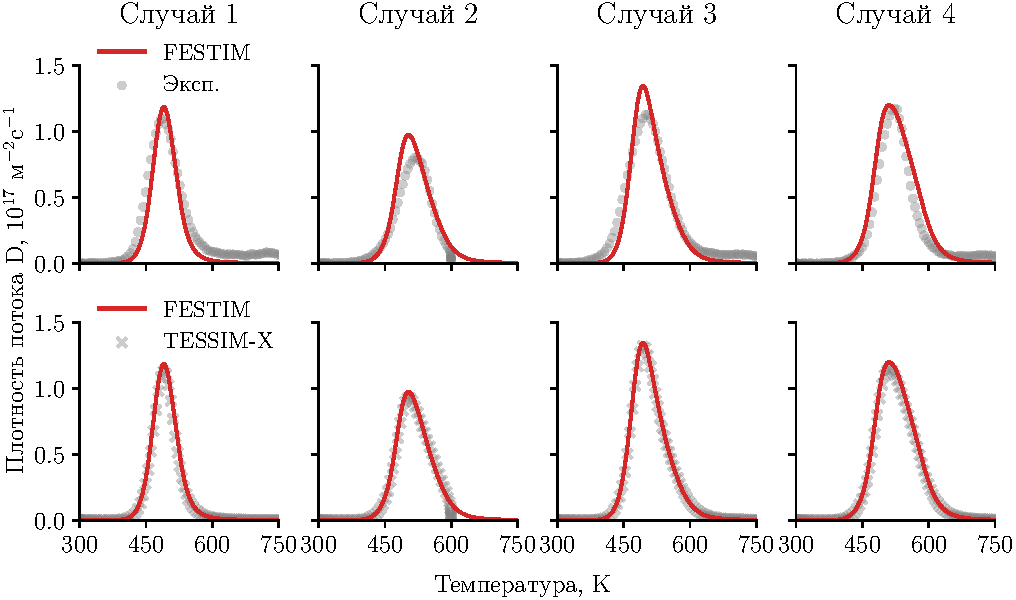
\includegraphics[scale=1]{val4.pdf}
    }
    \caption{ТДС-спектры дейтерия из разных образцов стали EUROFER. Сравнение с экспериментальными данными (вверху) и результатами моделирования в коде TESSIM-X (внизу)}\label{fig:ch2/val4}
\end{figure}

Наличие индуцированных центров захвата немного сдвигает основные пики ТДС-спектров в область более высоких температур. Их присутствие также приводит к уширению профиля, характеризующегося более плавно спадающим высокотемпературным плечом. Хотя согласие между результатами FESTIM и экспериментальными данными (верхний ряд на рис.~\ref{fig:ch2/val4}) является удовлетворительным (среднеквадратическое отклонение составляет \SI{7.9e15}{\per\meter\squared\per\second}), корреляция с TESSIM-X (нижний ряд на рисунке) является превосходной. Незначительные расхождения можно отнести к различиям в реализациях модели, учитывающей процессы на поверхности, а также в некоторых входных параметрах, которые восстановить не удалось.

\section{Выводы к главе 2}

Программный пакет FESTIM является апробированным инструментом для моделирования транспорта изотопов водорода в материалах на основе модели Макнабба и Фостера. При определяющем участии автора в коде была реализована гибкая модель, которая позволяет явно учитывать эволюцию концентрации адсорбированного водорода за счет обратимых процессов перехода между растворенным и адсорбированным состояниями, а также различных каналов адсорбции и десорбции. 

Возможности модели, учитывающей процессы на поверхности, были продемонстрированы успешным воспроизведением результатов четырех экспериментальных работ. Моделирование показали хорошее согласие с экспериментальными данными при различных предположениях относительно объемных и поверхностных процессов, влияющих на динамику водорода в материалах, что существенно расширяет область применения кода FESTIM. Верификация и высокая корреляция результатов с другими расчетными кодами (MHIMS и TESSIM-X) подтвердили аккуратность имплементации модели.

\nomenclature[A, 13]{MMS}{Метод построенных решений (Method of manufactured solutions)}

\FloatBarrier
